\chapter{User Documentation - Library}

This chapter describes how to use the NextGen SPICE simulator, and provides the guidelines for adding new circuit analyses and device types. The necessary binaries are available in the \texttt{/binaries} folder on the attached CD for copying. 

\section{Tutorials}
This sections shows the usage of the library on simple examples to present the basic idea of how to use the NextGen SPICE library. All these examples will use the .NET Core Console Application project template. The project should reference the \texttt{NextGenSpice.Core} assembly for circuit description, \texttt{NextGenSpice.Parser} assembly for parser implementation, \texttt{NextGenSpice.LargeSignal} assembly for the actual simulator, and all assemblies with the \texttt{System.Composition} preffix from the \texttt{/binaries} folder. Also, \texttt{NextGenSpice.Numerics.Native.dll} needs to be copied to the same folder as the compiled executable. We will use gnuplot \cite{gnuplot} to create the plots of the simulation results, so reader should have it installed as well.

\subsection{Calculating DC Bias of the Ciruit}
Suppose we wanted to calculate node voltages in the circuit shown in figure \ref{fig:userdocs:simple-circuit}.

\begin{figure}[h]
	\centering
	\begin{circuitdev}
		(0,0) 
		to[V=12<\volt>,invert] (3,0) node[label={-90:$1$}]{}
		-- (6,0)
		to[R, l=5<\ohm>, .-*] (6,3) node[label={3:$3$}]{}
		to[R, l=5<\ohm>] (3,3) node[label={$2$}]{}
		to[R, l=10<\ohm>] (0,3)
		-- (0,0)
	
		(3,0) to[R, l=10<\ohm>, *-*] (3,3)
		(0,1.5) -- (-0.5,1.5) node[ground]{}
	\end{circuitdev}
	\caption{Example circuit}
	\label{fig:userdocs:simple-circuit}
\end{figure}

Before we start with the actual analysis, we first need to construct the circuit representation. This is done using the \texttt{CircuitBuilder} class. Following code fragment constructs the circuit description of our circuit.

\begin{csharpcode}
// requires NextGenSpice.Core.Circuit and
// NextGenSpice.Core.Devices namespace
var builder = new CircuitBuilder();
builder
	.AddDevice(new[] {1, 0}, new VoltageSource(12))
	.AddDevice(new[] {0, 2}, new Resistor(10))
	.AddDevice(new[] {1, 2}, new Resistor(10))
	.AddDevice(new[] {2, 3}, new Resistor(5))
	.AddDevice(new[] {1, 3}, new Resistor(5));
var circuit = builder.BuildCircuit();
\end{csharpcode}

For convenience, class \texttt{CircuitBuilderExtensions} defines extensions methods that can be used to make the code more readable. The circuit can be equivalently created by the following code.

\begin{csharpcode}
// extensinos are contained in 
// NextGenSpice.Core.Extensions namespace
var builder = new CircuitBuilder();
builder
	.AddVoltageSource(1, 0, 12)
	.AddResistor(0, 2, 10)
	.AddResistor(1, 2, 10)
	.AddResistor(2, 3, 5)
	.AddResistor(1, 3, 5);
var circuit = builder.BuildCircuit();
\end{csharpcode}

The \texttt{circuit} object created in the preceding code fragments is only a description of the circuit. In the next step, we use it to create it's large-signal model, which we will use to perform the actual analysis.

\begin{csharpcode}
// requires NextGenSpice.LargeSignal namespace
// equivalent to
// var m = AnalysisModelCreator
//     .Instance.Create<LargeSignalCircuitModel>(circuit);
var model = circuit.GetLargeSignalModel();
\end{csharpcode}

The call to the method \texttt{EstablishDcBias} performs the actual node voltage calculation. Calculated node voltages can be found in an array in \texttt{LargeSignal\+CircuitModel.NodeVoltages} property.

\begin{csharpcode}
model.EstablishDcBias();
Console.WriteLine(model.NodeVoltages[1]); // 12 
Console.WriteLine(model.NodeVoltages[2]); //  8 
Console.WriteLine(model.NodeVoltages[3]); // 10 
\end{csharpcode}

The simulator also automatically calculates data for individual devices, and stores them in their large-signal model instances contained in the \texttt{LargeSignal\+CircuitModel.Devices} collection. In our case, all currents flowing through the circuit devices are calculated. As an example, we show how to get value of current flowing through the voltage source in our circuit. 

First, we need to identify the device in the collection. This can be done by providing a \textit{tag} parameter during the circuit representation construction. Arbitrary object can be used as a tag, we will use a string tag.

\begin{csharpcode}
builder
	.AddVoltageSource(1, 0, 12, "VS")
//	equivalent to
//  .AddDevice(new[] { 1, 0 }, new VoltageSourceDevice(12, "VS"))
	...
\end{csharpcode}

This tag is then used to query the \texttt{LargeSignalCircuitModel.Devices} collection, which stores the implementations of \texttt{ILargeSignalDevice} interface for each circuit from the description. For convenience, each analysis model defines method \texttt{FindDevice()} to simplify the syntax.

\begin{csharpcode}
// requires NextGenSpice.LargeSignal.Devices namespace
// equivalent to
// var vsource = (ITwoTerminalLargeSignalDevice) model.Devices
//	.SingleOrDefault(dev => Equals(dev.DefinitionDevice.Tag, "VS"));
var vsouce = (ITwoTerminalLargeSignalDevice) model.FindDevice("VS");
Console.WriteLine(vsouce.Current); // -0.8
\end{csharpcode}

The casting to \texttt{ITwoTerminalLargeSignalDevice} interface is necessary, because some circuit devices may have more than two terminals (e.g. transistors), and the Current property would note make sense for them. The whole example example then reads as follows:

\begin{csharpcode}
var builder = new CircuitBuilder();
builder
.AddVoltageSource(1, 0, 12, "VS")
.AddResistor(0, 2, 10)
.AddResistor(1, 2, 10)
.AddResistor(2, 3, 5)
.AddResistor(1, 3, 5);
var circuit = builder.BuildCircuit();

var model = circuit.GetLargeSignalModel(); ;
model.EstablishDcBias();

Console.WriteLine(model.NodeVoltages[1]); // 12
Console.WriteLine(model.NodeVoltages[2]); //  8
Console.WriteLine(model.NodeVoltages[3]); // 10

var vsouce = (ITwoTerminalLargeSignalDevice) model.FindDevice("VS");
Console.WriteLine(vsouce.Current); // -0.8
\end{csharpcode}

\subsection{Performing Transient Analysis}
\label{chap:tutorial-transient}
In previous section, we showed how to use the library to compute DC Bias of the circuit. Now we will show how to perform transient analysis. Consider the circuit shown in figure \ref{fig:userdocs:rlc-circuit}.

\begin{figure}[h]
	\centering
	\begin{circuitdev}
		(0,0) node[ground]{}
		to[V=5<\volt>, -*, invert] (0, 3) node[label=135:1]{}
		to[R=50<\ohm>] (3, 3) node[label=3:2]{}
		to[L=0.125<\henry>, *-*] (3, 0) node[label=305:3]{}
		to[C=1<\micro\farad>] (0, 0)
	\end{circuitdev}
	\caption{Simple series RLC circuit.}
	\label{fig:userdocs:rlc-circuit}
\end{figure}

We will calculate how the circuit behaves if the 5 V from the voltage source come in a sudden pulse. The NextGen SPICE library supports many input source behaviors, the full list can be found in section \ref{chap:devdocs:devices}. We will specify the desired behavior by passing an instance of \texttt{PulseBehavior} to voltage source when building the circuit. 

\begin{csharpcode}
var circuit = new CircuitBuilder()
	// behaviors are located in NextGenSpice.Core.BehaviorParams namespace
	.AddVoltageSource(1, 0, new PulseBehavior()
	{
		InitialLevel = 0,
		PulseLevel = 5,
		Delay = 5e-3, // 5 ms
		PulseWidth = 25e-3 // 25 ms
	})
	.AddResistor(1, 2, 50)
	.AddInductor(2, 3, 0.125)
	.AddCapacitor(3, 0, 1e-6)
	.BuildCircuit();
\end{csharpcode}

Then, as in the previous example, we get the \texttt{LargeSignalCircuitModel} and calculate the initial state of the circuit using the \texttt{EstablishDcBias()} method. After that, we can call the \texttt{AdvanceInTime()} method to perform the timesteps. Following code fragment can be then used to print voltage values of nodes 1 and 3 over time.

\begin{csharpcode}
var model = circuit.GetLargeSignalModel();
model.EstablishDcBias();

Console.WriteLine("Time V(1) V(3)");

var timestep = 0.2e-3; // use 0.2 ms timestep
while (model.CurrentTimePoint <= 55e-3) // simulate for 55 ms
{
	var time = model.CurrentTimePoint;
	var v1 = model.NodeVoltages[1];
	var v3 = model.NodeVoltages[3];
	
	Console.WriteLine($"{time} {v1} {v3}");
	
	model.AdvanceInTime(timestep);
}
\end{csharpcode}

If we redirect the program output to a file named \texttt{output.txt}, we can run gnuplot and use following commands to create a \texttt{plot.svg} file with plot of the voltage values over time as shown in figure \ref{fig:userdocs:rlc-plot}.

\begin{minted}[linenos, tabsize=4, fontsize=\footnotesize]{gnuplot}
set terminal svg size 600, 250
set output 'plot.svg'
set key autotitle columnhead
set xlabel 'Time'
set ylabel 'Value'
set grid ytics lt 0 lw 1 lc rgb '#bbbbbb'
set grid xtics lt 0 lw 1 lc rgb '#bbbbbb'
plot for [i=2:3] 'output.txt' using 1:i with lines
\end{minted}


\begin{figure}[h]
	\centering
	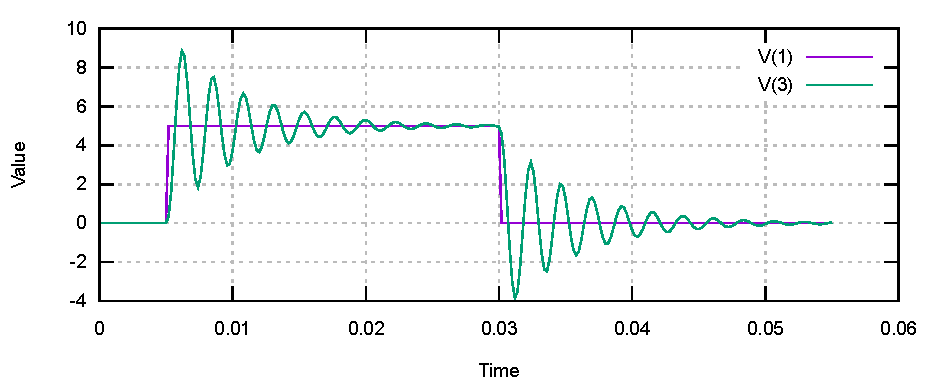
\includegraphics[width=0.8\linewidth]{04-fig-rlc-plot}
	\caption{Results on the RLC circuit.}
	\label{fig:userdocs:rlc-plot}
\end{figure}

\subsection{Loading Circuits from Netlists}

The NextGen SPICE library supports loading circuit description from SPICE netlist files. The supported syntax is shown in chapter \ref{chap:spicecode}. We will demonstrate this on the circuit shown in figure \ref{fig:back-to-back-circuit}. This is the same circuit we have shown earlier in the introduction chapter because of it's $1\mu\Omega$ resistor.

\begin{figure}[h]
	\begin{subfigure}{0.44\linewidth}
		\begin{spicecode}
Back to Back diodes
*
V1 IN 0 SIN(0 5 100 0 0 0)
D1 IN A D1N4148
R1 A B 1e-6
D2 0 B D1N4148
*
.MODEL D1N4148 D (
+ IS=2.52e-9 N=1.752 TT=2e-8
+ CJO=9e-13 M=0.25 VJ=20 BV=75
+ RS=0.568)
		\end{spicecode}
	\end{subfigure}
	\begin{subfigure}{0.55\linewidth}
	
		\centering
		\begin{circuitdev}
			(0,0) node[ground]{} -- (-2,0)
			to[sV<=5<\volt>,a=\text{V1 100Hz}] (-2,6) -- (0,6) node[circ,label=IN]{} -- (2,6)
			to[D,a=D1, l=D1N4148] (2,4) node[label=1:A]{} to[R=1<\micro\ohm>, a=R1, *-*] (2,2) node[label=1:B]{} to[D,invert, a=D2, l=D1N4148] (2,0) -- (0,0)
		\end{circuitdev}
	\end{subfigure}
	\caption{Back to back diode circuit and corresponding netlist}
	\label{fig:back-to-back-circuit}
\end{figure}

When imported from a netlist file, each device is automatically tagged by its name in uppercase letters so that it can be found among the other devices. Following code fragments prints the current flowing through the \texttt{D1} diode, and figure \ref{fig:04-fig-back-to-back-gear} shows the plot of the data.

\begin{csharpcode}
// parser is located in NextGenSpice.Parser namespace

// import circuit definiton from the file
var parser = SpiceNetlistParser.WithDefaults();
var result = parser.Parse(new StreamReader("circuit.cir"));
var circuit = result.CircuitDefinition;

// get simulation model
var model = circuit.GetLargeSignalModel();
var d1 = (ITwoTerminalLargeSignalDevice) model.FindDevice("D1");
var inNode = result.NodeIndices["IN"];

Console.WriteLine("Time V(IN) I(D1)");

var timestep = 10e-6; // use 10 us timestep
while (model.CurrentTimePoint <= 10e-3) // simulate for 10 ms
{
	var time = model.CurrentTimePoint;
	var vin = model.NodeVoltages[inNode];
	var id1 = d1.Current;
	
	Console.WriteLine($"{time} {vin} {id1}");
	
	model.AdvanceInTime(timestep);
}
\end{csharpcode}

\begin{figure}[h]
	\centering
	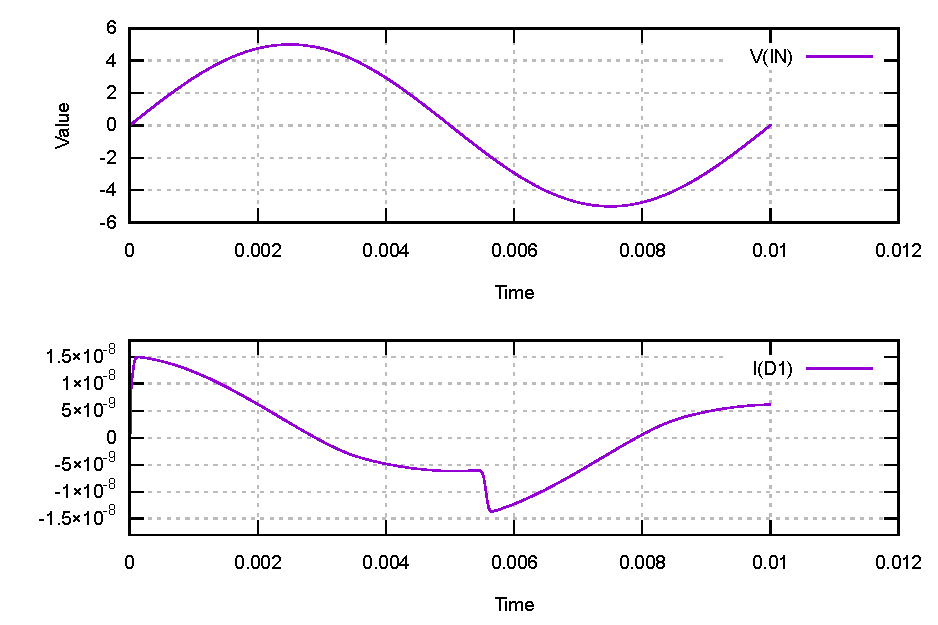
\includegraphics[width=.85\linewidth]{04-fig-back-to-back-gear}
	\caption{Plot of simulation output of back-to-back diode circuit.}
	\label{fig:04-fig-back-to-back-gear}
\end{figure}

\subsection{Defining a Subcircuit in Source Code}

NextGen SPICE support defining a custom subcircuit, which then can be used multiple times throughout the circuit and even in different circuits. In this tutorial, we will define a subcircuit representing a $9V$ battery with $1.5\Omega$ internal resistance, which is modelled as $9V$ voltage source and $1.5\Omega$ resistor in series, as shown in figure \ref{fig:userdocs:battery}.

\begin{figure}[h]
	\begin{circuitdev}
		(0,0) node[circ,label=N-]{} to[V=9<\volt>, invert] (3,0) to[R=1.5<\ohm>] (6,0) node[circ,label=N+]{}
	\end{circuitdev}
	\caption{Subcircuit for $9V$, $1.5\Omega$ battery}
	\label{fig:userdocs:battery}
\end{figure}

The subcircuit is created using the \texttt{CircuitBuilder} class, just as if it were a normal circuit, only instead of \texttt{BuildCircuit()} method, the \texttt{BuildSubcircuit()} method needs to be called with an array specifying which subcircuit nodes should be treated as terminals. The battery definition then can be used as an argument to \texttt{AddSubcircuit()} extension method, or passed to the \texttt{SubcircuitDevice} class constructor. Following code fragment constructs part of a circuit with two $9V$ batteries in series.

\begin{csharpcode}
var builder = new CircuitBuilder();
var batteryDefinition = builder
	.AddVoltageSource(1, 2, 9)
	.AddResistor(2, 3, 1.5)
	.BuildSubcircuit(new [] {1, 3});

builder.Clear();
builder
	.AddDevice(new[] {0, 1}, new Subcircuit(batteryDefinition))
	.AddSubcircuit(new[] {1, 2}, batteryDefinition);
	...
\end{csharpcode}


It is also possible to inspect the state of the devices inside the subcircuit during simulation. The \texttt{SubcircuitDevice}'s counterpart in \texttt{LargeSignalDeviceModel\+.Devices} implements \texttt{ILargeSignalSubcircuit} interface, which exposes the devices inside via the \texttt{Devices} property.

In this section, we described the usage of the simulator on simple examples, in next section, we revisit individual parts of the simulator and provide detailed description of it's interface.

\section{NextGenSpice.Core}

The \texttt{NextGenSpice.Core} assembly contains the analysis independent parts of the NextGen SPICE library, namely the classes for circuit description, and logic for validating the circuit.

\subsection{Creating the Circuit Description}
As we briefly described in the tutorials in previous section. The NextGen SPICE library works by first creating an analysis-independent \texttt{CircuitDefinition} class, which is then transformed into the analysis-dependent circuit model. The description of the circuit (the \texttt{CircuitDefinition} class) is created using the \texttt{Circuit\+Builder} class using the \texttt{Add(int[] terminals, ICircuitDefinitionDevice device)} method. The circuit builder then saves the reference to the device and sets node connections appropriately. If multiple copies of the same device should be added to the circuit, it is necessary to clone the device via the \texttt{ICircuitDefinitionDevice.Clone} method.

For convenience, there is a static class \texttt{CircuitBuilderExtensions} which contains extension methods on \texttt{CircuitBuilder} like \texttt{AddResistor}, \texttt{AddDiode} etc., which can be used to shorten the code that adds the individual devices.

\subsection{Supported Circuit Devices}
\label{chap:devdocs:devices}
Following table lists devices available in the NextGen SPICE simulation library. 

\begin{center}
	\begin{tabular}{|l|l|l|}
		\hline
		Device & Nodes & Parameters \\ \hline \hline
		\texttt{Resistor} & $N_+$, $N_-$ & Resistance \\ \hline
		\texttt{Capacitor} & $N_+$, $N_-$ & Capacitance, initial voltage \\ \hline
		\texttt{Inductor} & $N_+$, $N_-$ & Inductance, initial current \\ \hline
		\texttt{VoltageSource} & $N_+$, $N_-$ & Voltage or \texttt{InputSourceBehavior} \\ \hline
		\texttt{CurrentSource} & $N_+$, $N_-$ & Current or \texttt{InputSourceBehavior} \\ \hline
		\texttt{Vccs} & $N_+$, $N_-$, $N_{Ref+}$, $N_{Ref-}$ & Gain \\ \hline
		\texttt{Vcvs} & $N_+$, $N_-$, $N_{Ref+}$, $N_{Ref-}$ & Gain \\ \hline
		\texttt{Cccs} & $N_+$, $N_-$ & \texttt{VoltageSource}, gain \\ \hline
		\texttt{Ccvs} & $N_+$, $N_-$ & \texttt{VoltageSource}, gain \\ \hline
		\texttt{Diode} & $N_+$, $N_-$ & \texttt{DiodeParam} \\ \hline
		\texttt{Bjt} & $N_{C}$, $N_{B}$, $N_{E}$, $N_{S}$ & \texttt{BjtParam} \\ \hline
	\end{tabular}
\end{center}

The parameters listed in the table are set in the class constructor and directly map to the SPICE netlist statement parameters which were described in depth in section \ref{chap:spicecode-devices}. The \texttt{DiodeParam} and \texttt{BjtParam} classes encapsulate the model parameters for the diode and BJT devices, and again map to the same parameters as in the netlist \texttt{.MODEL} parameters. Additionally, each device class accepts an optional \texttt{object} parameter as its tag.

The \texttt{InputSourceBehavior} class is the base class for several source behavior specification classes. Again, these classes directly map to the transient input sources from the SPICE netlist syntax, as described in \ref{chap:spicecode-input-sources}. The supported behaviors are listed in the following table.

\begin{center}
	\begin{tabular}{|l|l|l|}
		\hline
		Behavior class & Netlist & Description \\ \hline \hline
		\texttt{ConstantBehavior} & DC & Constant input source value \\ \hline
		\texttt{SinusoidalBehavior} & SIN & Sinusoidal source \\ \hline
		\texttt{PieceWiseLinearBehavior} & PWL & Arbitrary piece-wise linear source \\ \hline
		\texttt{PulseBehavior} & PULSE & Source with regular pulses  \\ \hline
		\texttt{ExponentialBehavior} & EXP & Source with exponential edges \\ \hline
		\texttt{AmBehavior} & AM & Amplitude modulated source \\ \hline
		\texttt{SffmBehavior} & SFFM & Single frequency modulated source \\ \hline
	\end{tabular}
\end{center}

\subsection{Creating Analysis-Specific Circuit Models}

Before any circuit analysis can be performed, the circuit definition must be transformed into the analysis-specific circuit model. NextGen SPICE currently supports only the \texttt{LargeSignalCircuitModel} which will be described in section \ref{chap:userdocs-large-signal} in more detail.

The circuit models are created using the \texttt{AnalysisModelCreator} class and its instance method \texttt{GetModel<TCircuitModel>(ICircuitDescription)}. This class encapsulates \texttt{IAnalysisModelFactory<TCircuitModel>} implementations for individual analysis model types. Factory implementations for analysis models provided by NextGen SPICE library are automatically registered using the MEF framework. These factories can be configured to use specific implementations for individual circuit devices. The configuration is done on the factory itself, which can be obtained using the \texttt{AnalysisModelCreator.GetFactory<TCircuit\+Model>()}.

There is a global instance of the \texttt{AnalysisModelCreator} class available at \texttt{AnalysisModelCreator.Instance} property. There is also an extension method on the \texttt{ICircuitDefinition} interface which uses the global model creator to create the \texttt{LargeSignalCircuitModel}, which can be used to simplify the code.

\section{NextGenSpice.Parser}
The NextGenSpice.Parser assembly contains the implementation of the SPICE netlist parser. The parser itself is represented by the \texttt{SpiceNetlistParser} class. The parser is designed to be extensible by registering statement processors for individual netlist statements, which will be covered later. An instance of the parser can be obtained via static methods \texttt{SpiceNetlistParser.Empty()} which return an instance of the parser without any statement processors registered, and \texttt{SpiceNetlistParser.WithDefaults()} which returns instance with handlers for all devices implemented in the NextGen SPICE library.

The parsing itself is done using the \texttt{Parse} method which returns an instance of \texttt{SpiceNetlistParserResult} which contains following properties:

\begin{itemize}
	\item \texttt{CircuitDefinition} -- Definition of the circuit contained in the netlist.
	\item \texttt{Subcircuits} -- Collection of \texttt{ISubcircuitDefinition} classes for the subcircuits defined in the top-level of the netlist (Subcircuits defined inside another subcircuit are not returned).
	\item \texttt{Models} -- collection of device model (parameter sets) defined in the netlist (again, models defined inside a subcircuit are not returned).
	\item \texttt{Title} -- The content of the title statement from the netlist.
	\item \texttt{Errors} -- Collection of \texttt{SpiceParserError} classes which wrap the errors encountered during the parsing.
	\item \texttt{NodeNames} -- NextGen SPICE uses \texttt{int} type to store the id of a node, this array can be indexed by the node id to obtain the string name that was used in the netlist. 
	\item \texttt{NodeIndices} -- Dictionary providing the inverse mapping to \texttt{NodeNames} property.
	\item \texttt{OtherStatements} -- Collection of \texttt{SpiceStatement}s that can be used to return user-defined statements from the parser.
\end{itemize}

To simplify obtaining references to individual circuit device instances, each instance has been tagged with the uppercase name of the device used in the netlist, so that a particular device can be easily obtained by \texttt{FindDevice} methods on circuit definition and circuit models.


\section{NextGenSpice.LargeSignal}
\label{chap:userdocs-large-signal}

The \texttt{NextGenSpice.LargeSignal} assembly contains the implementation of the large-signal circuit model which is used to perform transient analysis of circuits. The simulation functionality is exposed through the \texttt{LargeSignalCircuitModel} class, and its \texttt{EstalblishDcBias} and \texttt{AdvanceInTime} instance methods. The \texttt{EstablishDcBias} method is used to calculates the DC bias of the circuit at initial timepoint, and \texttt{AdvanceInTime} method is used to get the DC bias after given timestep.

\subsection{Accessing the Computed State}
The calculated node voltages are stored in an array in the \texttt{NodeVoltages} property on the \texttt{LargeSignalCircuitModel} class. The \texttt{Devices} property stores large-signal representation classes as \texttt{ILargeSignalDevice} instances for the devices used in the circuit. These instances can be used to inspect the state computed for each circuit device. The \texttt{ILargeSignalDevice} instance for a particular device can be obtained by using the \texttt{FindDevice} method, which has overloads accepting \texttt{ICircuitDefinitionDevice} instance, or an \texttt{object} which was used as a tag during circuit construction. The state is exposed in two ways: \texttt{GetDeviceState\+Providers} method returning a collection of \texttt{IDeviceStateProvider} classes, and through the individual properties on the device implementation instance.

The \texttt{IDeviceStateProvider} instances can be used to print all the available state variables. The \texttt{Name} property gives the name of the variable, like "I" for the current flowing through the device, and \texttt{GetValue} method can be used to obtain the respective value.

The same state can be accessed through individual properties on the device implementation class instance. For example, in case of two terminal devices like resistor or voltage source, the respective class implements the \texttt{ITwoTerminalLarge\+SignalDevice} interface, which exposes \texttt{Voltage} and \texttt{Current} property containing the voltage across the device and current flowing through the device, respectively. The \texttt{ITwoTerminalLargeSignalDevice} interface is implemented by all implemented devices except the BJT transistor.

The BJT transistor implementation class \texttt{LargeSignalBjt} exposes properties \texttt{CurrentBase}, \texttt{CurrentCollector} and \texttt{CurrentEmitter} which expose the currents flowing through the respective terminals, and \texttt{VoltageBaseCollector}, \texttt{VoltageBaseEmitter} and \texttt{VoltageCollector\+Emitter} for voltages between individual pairs of terminals.

\subsection{Modifying the Device Parameters}
The device's implementation used in the \texttt{LargeSigalCircuitModel} retain references to the corresponding circuit definition classes. This means that changes made to the device parameters inside \texttt{CircuitDefinition} are reflected in the next DC bias point calculation. To demonstrate, recall the circuit we used in the DC Bias calculation tutorial (figure \ref{fig:userdocs:simple-circuit}). The following code snippet prints the DC bias values for increasing values of the rightmost resistor.

\begin{csharpcode}
// build circuit	
var builder = new CircuitBuilder();
builder
	.AddVoltageSource(1, 0, 12, "VS")
	.AddResistor(0, 2, 10)
	.AddResistor(1, 2, 10)
	.AddResistor(2, 3, 5)
	.AddResistor(1, 3, 5, "R1");
var circuit = builder.BuildCircuit();
var model = circuit.GetLargeSignalModel();
var vsouce = (ITwoTerminalLargeSignalDevice)model.FindDevice("VS");
var res = (ResistorDevice)circuit.FindDevice("R1");

// sweep for values from 1 Ohm to 15 Ohm
for (int i = 1; i <= 15; i++)
{
	res.Resistance = i+1; // set resistance
	
	// calculate
	model.EstablishDcBias();
	var v1 = model.NodeVoltages[1];
	var v2 = model.NodeVoltages[2];
	var v3 = model.NodeVoltages[3];
	var iV = vsouce.Current;
	
	// print values
	Console.WriteLine($"{i+1}Ohm: {v1}V {v2}V {v3}V {iV}A");
}
\end{csharpcode}

\subsection{Changing the Integration Method}
Some circuits are sensitive to the choice of numerical integration method used during the simulator. The default integration method is GEAR-2 method, which is a reasonable compromise between accuracy and stability. However, use of GEAR-2 method dampens the oscilations of RLC circuits. Consider the trivial circuit in figure \ref{fig:oscillation-circuit}. Because this circuit lacks any resistance, the voltage at node 1 should oscillate indefinitely with amplitude of 1V.

\begin{figure}[h]
	\centering
	\begin{circuitdev}
		(0,0) node[circ,label=1]{} -- (-1,0) to[C, a=1<\nano\farad>] (-1,-3) -- (0,-3) node[ground]{} -- (1,-3)  to[L, a=1<\micro\henry>,i_=\mbox{$i=1mA$}] (1,0) -- (0,0)
	\end{circuitdev}
	\caption{Indefinitely oscillating circuit}
	\label{fig:oscillation-circuit}
\end{figure}

However, the GEAR-2 method dampens the oscillation. The simulator results with GEAR-2 method are shown in figure \ref{fig:oscillation-gear}

\begin{figure}[H]
	\centering
	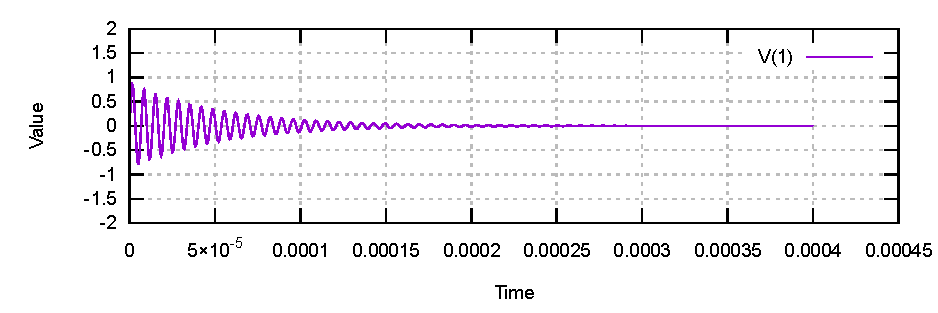
\includegraphics[width=.85\linewidth]{oscillation-gear}
	\caption{Simulation results on oscillating circuit using GEAR-2 method}
	\label{fig:oscillation-gear}
\end{figure}

For comparison, the figure \ref{fig:oscillation-trap} shows the same simulation with trapezoidal integration method.

\begin{figure}[h]
	\centering
	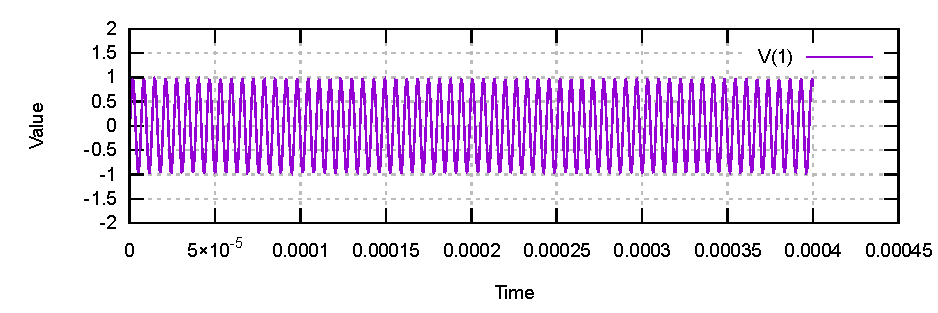
\includegraphics[width=.85\linewidth]{oscillation-trap}
	\caption{Simulation results on oscillating circuit using trapezoidal rule}
	\label{fig:oscillation-trap}
\end{figure}

Even though the trapezoidal method is more precise in terms of smaller local truncation error and does not dampen the oscillations, it is less stable than other methods. For comparison figure \ref{fig:04-fig-back-to-back-trap} shows plots of data obtained using the trapezoidal rule on the back-to-back diode circuit we have shown back in figure \ref{fig:back-to-back-circuit}. Notice the numerical noise, also known as \textit{trapezoidal ringing}, present in the plot.\footnote{We have increased the timestep to $100\mu{}s$, the original $10\mu{}s$ timestep also produces numerical oscilation, but due to the density of the oscilation the plot would be merged into a single thick line.}

\begin{figure}[h]
	\centering
	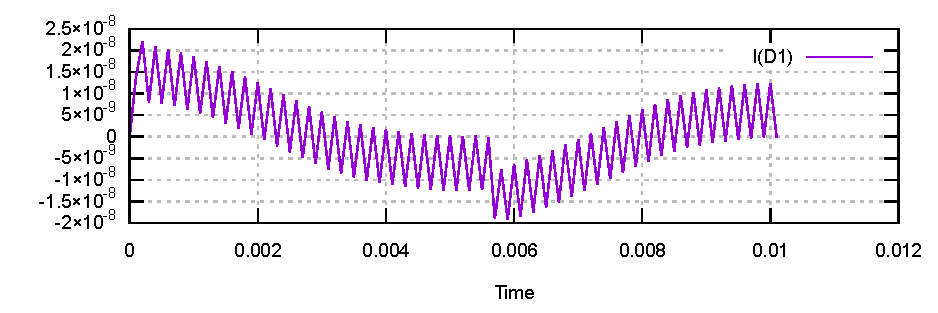
\includegraphics[width=.85\linewidth]{04-fig-back-to-back-trap}
	\caption{Simulation results of back-to-back diode using the trapezoidal rule}
	\label{fig:04-fig-back-to-back-trap}
\end{figure}

The numerical method that is used during the simulation can be changed by replacing the \texttt{IntegrationMethodFactory} property on \texttt{LargeSignalCircuit\+Model.CircuitParameters} object. Following code fragment shows how to configure the simulator to use the Trapezoidal Rule integration method.

\begin{csharpcode}
LargeSignalCircuitModel model = /* ... */;

// requires NextGenSpice.LargeSignal.NumIntegration namespace
model.CircuitParameters.IntegrationMethodFactory =
	new SimpleIntegrationMethodFactory(
		() => new TrapezoidalIntegrationMethod());
\end{csharpcode}

The supported integration methods are listed in the following table

\begin{center}
	\begin{tabular}{|l|l|}
		\hline
		Integration method & Class name \\ \hline \hline
		GEAR method & \texttt{GearIntegrationMethod} \\ \hline
		Trapezoidal rule & \texttt{TrapezoidalIntegrationMethod} \\ \hline
		Backward (implicit) Euler & \texttt{BackwardEulerIntegrationMethod} \\ \hline
		Adams Moulton & \texttt{AdamsMoultonIntegrationMethod} \\ \hline
	\end{tabular}
\end{center}

\chapter{Extending the Library}
\label{chap:exteding}
This chapter describes the functionality of the library can be extended by the user. Also, in section \ref{chap:userdocs:diode-tutorial}, we provide an example code that implements a simple diode device that will demonstrate the process on a concrete example.

\section{Adding New Circuit Devices}
Adding new circuit devices requires both creating a class that is used in circuit description and class that implements the actual large-signal simulation logic. We will describe both parts in separate subsections.

\subsection{Adding Device Description}

Each device description class must implement the \texttt{ICircuitDefinitionDevice} interface. To simplify the implementation of new devices, the library provides basic implementation of this interface in \texttt{CircuitDefinitionDevice} abstract class. Furthermore, there exists \texttt{TwoTerminalCircuitDevice} abstract class which defines additional member which can be useful for devices with two terminals. 

These classes can be then immediately used as arguments to the \texttt{Circuit\+Builder.AddDevice} method and thereby in the circuit definition. If the device should participate in the circuit topology validation, then the derived classes should override the \texttt{GetBranchMetadata} method and return the \texttt{CircuitBranch\+Metadata} instances that describe which terminals are connected by voltage-defined and current-defined branches.

\subsection{Adding Large-Signal Device Implementation}

To use these devices during a circuit analysis, their analysis-specific logic must be implemented and then registered in the respective \texttt{IAnalysisModelFactory} instance, so that the \texttt{AnalysisModelCreator} knows which implementation to use when creating the \texttt{LargeSignalCircuitModel}.

The Device's large-signal implementation needs to implement the \texttt{ILarge\+SignalDevice} interface. This interface defines following members:

\begin{itemize}
	\item \texttt{RegisterAdditionalVariables} -- Allows implementation to add additional variables to the equation system via supplied \texttt{IEquationSystemAdapter} instance.
	\item \texttt{Initialize} -- Lets devices request equation system proxies from \texttt{IEquation\+SystemAdapter}, and perform other necessary initialization, like getting numerical integrators from \texttt{ISimulationContex.SimulationParameters.\+IntegrationMethodFactory}.
	\item \texttt{ApplyModelValues} -- Applies devices MNA stamp into the equation system. If the device is nonlinear, the linearized equivalent circuit should be stamped.
	\item \texttt{OnEquationSolution} -- Lets devices check for solution convergence (compare current solution with the previous one). The tolerancies can be accessed in \texttt{ISimulationContext.SimulationParameters} object, and if the solution did not converge, the \texttt{ISimulationContext.ReportNotConverged} method should be called.
	\item \texttt{OnDcBiasEstablished} -- Called after the Newton-Raphson iterations have reached a fixed point and the calculation of the current timestep has completed.
\end{itemize}

The mapping between circuit definition classes and their analysis implementations is done for each analysis model separately by calling the \texttt{SetModel<TRep, TMod>} method on the respective \texttt{IAnalysis\+ModelFactory} instance. The method accepts a function which creates the implementation class from the circuit definition class. The following code snippet shows how to register \texttt{LargeSignal\+Resistor} as the implementation of \texttt{Resistor} device for \texttt{LargeSignalCircuit\+Model}.

\begin{csharpcode}
var factory = AnalysisModelCreator.Instance
	.GetFactory<LargeSignalCircuitModel>();

factory.SetModel<Resistor, LargeSignalResistor>(
	resistor => new LargeSignalResistor(resistor));
\end{csharpcode}

This mapping can be later changed by another call to \texttt{SetModel} method. It is also possible to create separate \texttt{AnalysisModelCreator} instances and have different mappings in each instance.

\section{Extending the Parser}

An optional step when adding a new device to the simulator is extending the parser to allow importing the new device from spice netlists.

\subsection{Adding New Device Processors}

The parser implemented in NextGen SPICE library delegates parsing of individual device statements to classes implementing the \texttt{IDeviceStatementProcessor} interface. Implementations of this interface can be added to the parser by calling the \texttt{RegisterDevice} method. We recommend creating new device statement processors by deriving from \texttt{DeviceStatementProcessor} abstract class. The derived class then needs to implement only the \texttt{Discriminator} char property which specifies the letter identifying the device (The letter should be uppercase), and \texttt{DoProcess} method that does the actual processing.

For simple devices with no dependencies, the \texttt{DoProcess} method may directly add the device to the \texttt{CircuitBuilder} accessible on the \texttt{protected} property of the same name in \texttt{DeviceStatementProcessor}. In case of devices like diode which depend on other statements (diode statement depends on \texttt{.MODEL} statement which defines its model parameters), the statement processing needs to be deferred until later. This is done by adding a \texttt{DeferredStatement} on the active \texttt{ParsingContext} accessible through the \texttt{Context} property of \texttt{DeviceStatement\+Processor} base class. The \texttt{DeferredStatement} defines the following methods.

\begin{itemize}
	\item \texttt{CanApply} -- Should return \texttt{true} if all dependencies of the statement have been processed and the statement can be processed next.
	\item \texttt{Apply} -- Should add the device into the circuit using the \texttt{CircuitBuilder} on the \texttt{ParsingContext}
	\item \texttt{GetErrors} -- Should return a collection of \texttt{SpiceParserErrors} that describe errors prevent the statement processing. This method is called once it is certain that no statement can be processed.
\end{itemize}

The \texttt{DeviceStatementProcessor} class also provides property \texttt{DeviceName} that exposes the name of the currently parsed device, and following methods.

\begin{itemize}
	\item \texttt{GetNodeIds(int start, int count)} -- Returns node ids of \texttt{count} nodes specified in the statement starting by token on with index \texttt{start}.
	\item \texttt{GetValue(int index)} -- parses the numeric value out of the token on \texttt{index}th token.
\end{itemize}

Both these method do the necessary error handling. The number of errors generated can be checked in the \texttt{Errors} property, and additional errors can be added to the \texttt{Context.Errors} collection. If no error is encountered, the processor should either add the device to the circuit using the \texttt{CircuitBuilder} property, or add a \texttt{DeferredStatement} to \texttt{Context.DeferredStatements} collection. The following code fragment shows how the resistor statements are parsed.

\begin{csharpcode}
protected override void DoProcess()
{
	var nodes = GetNodeIds(1, 2);
	var rvalue = GetValue(3);
	
	if (Errors == 0)
		CircuitBuilder.AddDevice(nodes, new Resistor(rvalue, DeviceName));
}
\end{csharpcode}

Because the resistor device does not depend on any other statement, the device can be added to the circuit straight away. In case of diode statements, diode devices cannot be added to circuit until the corresponding \texttt{.MODEL} statement is parsed. Because \texttt{.MODEL} statements are used to set parameters for many device types, there is a \texttt{ModeledDevice\+DeferredStatement<T>} class deriving from \texttt{DeferredStatement}. which implements the checking for models. This class is used in the \texttt{DiodeStatementProcessor} as shown in the following code fragment.

\begin{csharpcode}
protected override void DoProcess()
{
	var nodes = GetNodeIds(1, 2);
	// cannot check for model existence yet, defer checking for model later
	
	if (Errors > 0)	return;
	
	var name = DeviceName; // captured in lambda
	var modelToken = RawStatement[3];
	Context.DeferredStatements.Add(
		new ModeledDeviceDeferedStatement<DiodeParams>(
			scope: Context.CurrentScope,
			addFunc: (par, cb) => cb.AddDevice(nodes, new Diode(par, name)),
			modelNameToken: modelToken));	
}
\end{csharpcode}

\subsection{Adding New Model Types}

Some devices (like diode and BJT transistor) require a corresponding \texttt{.MODEL} statement. The SpiceNetlistParser therefore can be extended to parse new models for new devices. The handling of models for the device is done by returning \texttt{IDeviceModelHandler} instances that do the parsing. The library again supplies a abstract class \texttt{DeviceModelHandlerBase<TParam>} that implements the basic logic. Derived classed need only specify the mapping to the parameter names. We show an example implementation of the \texttt{IDeviceModelHandler} later in section \ref{chap:userdocs:diode-example:parser}.

\section{Example: Adding a Diode Device}
\label{chap:userdocs:diode-tutorial}

In previous sections we described all the steps needed to add a new device to the simulator. To provide a concrete example, we will show in this section how to implement a simple diode device. The NextGen SPICE library already contains diode device implementation, represented by classes \texttt{Diode} and \texttt{LargeSignalDiode}, which is more complex version of the one we will show in this section. The library is designed so that circuit description classes can be reused, and the new diode implementation would require implementing only the device's large-signal logic. However, to demonstrate how completely new devices can be added to the library, we will not reuse the existing diode class. Our diode will be modeled solely by the Shockley diode equation and parameters shown in figure \ref{fig:userdocs:tutorial:diode-params}. The names in capital letters will be later used in diode statements in SPICE netlists. 

\begin{figure}[h]
	\centering
	
	\[ I = I_S \left(e^{\frac{V}{n \cdot V_t}} - 1 \right) \]
	
	\begin{tabular}{|l|l|l|}
		\hline 
		Parameter & Name & Description \\ \hline \hline
		$I_S$ & IS & Saturation current \\ \hline
		$n$ & N & Ideality coefficient \\ \hline
		$V_t$ & VT & Thermal voltage \\ \hline
		
	\end{tabular}
	
	\caption{Shockley diode equation and its parameters for modeling the diode}
	\label{fig:userdocs:tutorial:diode-params}
\end{figure}


To differentiate from diode already implemented in the library, we will use the prefix \texttt{Shockley} for the classes implemented in this tutorial.

\subsection{Creating a Diode Device Definition}
First, we have to create a class implementing \texttt{ICircuitDescriptionDevice}, which will be used to represent the diode in the circuit description. Since diode has two terminals, we will derive our class from the \texttt{TwoTerminalDevice} class, which already implements members needed by the interface. The only thing we have to add are the diode parameters. To keep with the practice of encapsulating the device parameters in separate class for semiconductor devices, we will define classes \texttt{ShockleyDiode} and \texttt{ShockleyDiodeParams} as follows.

\begin{csharpcode}
public class ShockleyDiodeParams
{
	// specify default parameters
	
	public double SaturationCurrent { get; set; } = 1e-14;
	public double ThermalVoltage { get; set; } = 25.8563e-3;
	public double IdealityCoefficient { get; set; } = 1;
}

// requires .Core.Devices namespace
public class ShockleyDiode : TwoTerminalCircuitDevice
{
	public ShockleyDiodeParams Param { get; set; }
	
	public ShockleyDiode(ShockleyDiodeParams param, object tag = null) 
		: base(tag)
	{
		Param = param;
	}
}
\end{csharpcode}

\subsection{Parsing diode statements}
\label{chap:userdocs:diode-example:parser}

Next we will show how to extend the parser to handle the new device. Suppose our Shockley diode statement should be specified by following syntax.

\begin{code}
S<name> <anode> <cathode> <model name>
.MODEL <name> SHOCKLEY([IS=<val>] [N=<val>] [VT=<val>])
\end{code}

We will start with the \texttt{.MODEL} statement. Parsing \texttt{ShockleyDiode\+Params} from the \texttt{.MODEL} statement is done by a class deriving from \texttt{Device\+ModelHandler\+Base<T>} specialized on the \texttt{ShockleyDiodeParams} type. The mapping of individual properties is set in the constructor by calling the \texttt{Map} method as shown in the following code fragment.


\begin{csharpcode}
// requires NextGenSpice.Parser.Statements.Devices; namespace
private class ShockleyDiodeModelHandler
	: DeviceModelHandlerBase<ShockleyDiodeParams>
{
	public ShockleyDiodeModelHandler()
	{
		Map(p => p.SaturationCurrent, "IS");
		Map(p => p.ThermalVoltage, "VT");
		Map(p => p.IdealityCoefficient, "N");
	}
	
	public override string Discriminator => "SHOCKLEY";
	
	protected override ShockleyDiodeParams CreateDefaultModel()
	{
		return new ShockleyDiodeParams();
	}
}
\end{csharpcode}

Now we will create the actual Shockle diode statement processor by deriving from \texttt{DeviceStatementProcessor}. This class will also override the \texttt{GetModel\+StatementHandlers} method and return an instance of the \texttt{ShockleyDiodeModel\+Handler} class which we implemented above.

\begin{csharpcode}
public class ShockleyDiodeStatementProcessor : DeviceStatementProcessor
{
	public override char Discriminator => 'S';
	
	public ShockleyDiodeStatementProcessor()
	{
		MinArgs = MaxArgs = 3;
	}
	
	protected override void DoProcess()
	{
		var nodes = GetNodeIndices(1, 2); 
		// cannot check for model existence yet,
		// defer checking for model later		
		
		if (Errors == 0) // no errors in node names or device name
		{
			// use local variable to be captured in lambda
			var name = DeviceName;
			var modelToken = RawStatement[3];
			Context.DeferredStatements.Add(
				new ModeledDeviceDeferedStatement<ShockleyDiodeParams>(
					Context.CurrentScope,
					(par, cb) =>
						 cb.AddDevice(nodes, new ShockleyDiode(par, name)),
					modelToken));
		}
	}

	public override IEnumerable<IDeviceModelHandler>
		GetModelStatementHandlers()
	{
		return new[] { new ShockleyDiodeModelHandler() };
	}
}
\end{csharpcode}

We now can register this class to \texttt{SpiceNetlistParser}, which will use them when parsing the netlist files.

\begin{csharpcode}
var parser =  SpiceNetlistParser.WithDefaults();
parser.RegisterDevice(new ShockleyDiodeStatementProcessor());
\end{csharpcode}

\subsection{Implementing Large-Signal Diode Logic}
Lastly, we will implement the large-signal logic for the shockley diode as the \texttt{LargeSignalShockleyDiode}. We will derive our class from \texttt{TwoTerminalLarge\+SignalDevice<ShockleyDiode>} class which provides the basic members needed by the \texttt{ILargeSignalDevice} interface.

Our \texttt{ShockleyDiode} device has nonlinear I-V characteristic, which needs to be iteratively linearized, as described in section \ref{chap:analysis:transient-overview}. The large-signal logic should therefore liearize the I-V characteristic at the candidate DC bias point and enter the corresponding coefficients into the equation system. To simplify manipulation with \texttt{IEquationSystemCoefficientProxy} objects, we will use the \texttt{CurrentStamper} and \texttt{ConductanceStamper} classes, which encapsulate writing stamps for current source and resistor devices, which form the linearized diode equivalent model. Also, we will use the \texttt{VoltageProxy} wrapper which will read the anode and cathode node voltages and return their difference, which is the voltage across the diode. These classes will be initialized by calling the \texttt{Register} method with the \texttt{IEquationSystemAdapter} during the initialization phase.

\begin{csharpcode}
	// classes encapsulating the work with equation system coefficient proxies
	// requires NextGenSpice.LargeSignal.Stamping namespace
	private VoltageProxy voltage; // used to get voltage across the diode
	
	// stamping equivalent circuit model
	private CurrentStamper currentStamper;
	private ConductanceStamper conductanceStamper;
	
	public LargeSignalShockleyDiode(ShockleyDiode definitionDevice)
		: base(definitionDevice)
	{
		voltage = new VoltageProxy();
		currentStamper = new CurrentStamper();
		conductanceStamper = new ConductanceStamper();
	}
	
	public override void Initialize(IEquationSystemAdapter adapter,
	ISimulationContext context)
	{
		// get proxies
		voltage.Register(adapter, Anode, Cathode);
		currentStamper.Register(adapter, Anode, Cathode);
		conductanceStamper.Register(adapter, Anode, Cathode);
	}
\end{csharpcode}

The actual logic for writing the equation system coefficients is done in the \texttt{ApplyModelValues} method. We will use the \texttt{DeviceHelpers} class to calculate the linear equivalents of the diode, and then use the \texttt{Stamp} method on the stamper classes to write the coefficients into the equation system.

\begin{csharpcode}
	public override void ApplyModelValues(ISimulationContext context)
	{
		var Is = DefinitionDevice.Param.SaturationCurrent;
		var Vt = DefinitionDevice.Param.ThermalVoltage;
		var n = DefinitionDevice.Param.IdealityCoefficient;
		
		var Vd = voltage.GetValue();
		// calculates current through the diode and it's derivative
		DeviceHelpers.PnJunction(Is, Vd, Vt * n, out var Id, out var Geq);
		Current = Id; 
		
		// stamp the equivalent circuit
		var Ieq = Id - Geq * Vd;
		conductanceStamper.Stamp(Geq);
		currentStamper.Stamp(Ieq);
	}
\end{csharpcode}

Because the diode is a nonlinear device, the DC bias calculation needs to be iterated until the values are in the specified tolerances. The convergence check for nonlinear devices is done in the \texttt{OnEquationSolution} method. Also we will update the \texttt{Voltage} property so that the voltage across the diode can be accessed by the outside code once the calculation is completed.

\begin{csharpcode}
	public override void OnEquationSolution(ISimulationContext context)
	{   
		var newVoltage = voltage.GetValue();
		var abstol = context.SimulationParameters.AbsoluteTolerance;
		var reltol = context.SimulationParameters.RelativeTolerance;
		
		// Check if converged
		if (!MathHelper.InTollerance(newVoltage, Voltage, abstol, reltol))
		{
			// request additional DC bias iteration
			context.ReportNotConverged(this);
		}
		
		// update voltage for reading
		Voltage = newVoltage;
	}
\end{csharpcode}

 To use the \texttt{LargeSignalShockleyDiode} as the diode implementation in \texttt{Large\+SignalCircuitModel}, we need to register it in the \texttt{Analysis\+ModelCreator} instance used to create the circuit model.


\begin{csharpcode}
	// requires NextGenSpice.Core.Representation
	var factory = AnalysisModelCreator.Instance
		.GetFactory<LargeSignalCircuitModel>();
	factory.SetModel<ShockleyDiode, LargeSignalShockleyDiode>(
		e => new LargeSignalShockleyDiode(e));
\end{csharpcode}

This concludes the diode implementation, the whole example can be found in the  \texttt{/sources/SandboxRunner/DiodeImplExample.cs} file on the attached CD.

\chapter{User Documentation - Standalone Application}
This chapter describes how to use the NextGenSpice standalone application. To run the application, the user needs to have .NET Core Runtime version 2.0 or newer installed on their computer. The latest version of the .NET Core Runtime can be downloaded from the official website\footnote{\url{https://www.microsoft.com/net/download/Windows/run}}. Because the program is command line based, an external tool is needed for the visualization of the transient analysis output. For this purpose, we recommend downloading and installing gnuplot from the official website.\footnote{\url{http://www.gnuplot.info/download.html}}

The program's binaries can be found in the \texttt{/binaries} folder on the attached CD. Before the library can be used, the contents of the \texttt{/binaries} folder need to be copied to an appropriate location (in this text, we will assume that the files are copied to \texttt{C:\textbackslash{}NextGenSpice\textbackslash} folder). If everything is set correctly, following command should produced the output shown.

\begin{code}
C:\NextGenSpice> dotnet NextGenSpice.dll
Usage: dotnet NextGenSpice.dll <input file>
C:\NextGenSpice>
\end{code}

The program does accept exactly one argument: path to a file containing the circuit in SPICE netlist format, as described in chapter \ref{chap:spicecode}. The application reads all the statements in the file and reports back any errors encountered. If there are no errors, then individual circuit analyses are executed. First, the respective simulation statement is printed back to standard output, and after that the simulation results are printed. The output format is described in the following sections.

\subsubsection{.OP Statement Output Format}
In the operating point analysis, the output consists of series of \texttt{<variable> = <value>} pairs, each on separate line. If no \texttt{.PRINT} statement is specified, then all available data is printed.

To illustrate, consider following netlist file.

\begin{figure}[h]
	\centering
	\begin{subfigure}{.25\textwidth}
		\begin{spicecode}
BRIDGE-T CIRCUIT
*
VBIAS 1 0 12
R1 1 2 10
R2 2 0 10
R3 2 3 5
R4 1 3 5
*
.OP
.END
		\end{spicecode}		
	\end{subfigure}\hspace{5mm}
	\begin{subfigure}{.7\textwidth}	
		\centering	
		\begin{circuitdev}
			(0,0) 
			to[V=12<\volt>,invert,a=VBIAS] (3,0) node[label={-90:$1$}]{}
			-- (6,0)
			to[R, l=5<\ohm>, .-*, a=R4] (6,3) node[label={3:$3$}]{}
			to[R, l=5<\ohm>, a=R3] (3,3) node[label={$2$}]{}
			to[R, l=10<\ohm>, a=R2] (0,3)
			-- (0,0)
			
			(3,0) to[R, l=10<\ohm>, a=R1, *-*] (3,3)
			(0,1.5) -- (-0.5,1.5) node[ground]{}
		\end{circuitdev}
	\end{subfigure}	
\end{figure}

This file is available on the attached CD in \texttt{/examples/bridget.txt}. Copy this file to the \texttt{C:\textbackslash{}NextGenSpice\textbackslash} folder. Following code snippet shows how the NextGenSpice output for this netlist file.

\begin{code}
C:\NextGenSpice> dotnet NextGenSpice.dll bridget.txt
.OP
V(1) = 12
V(2) = 8
V(3) = 10

I(VBIAS) = -0.8
V(VBIAS) = 12

I(R1) = 0.4
V(R1) = 4

I(R2) = 0.8
V(R2) = 8

I(R3) = -0.4
V(R3) = -2

I(R4) = 0.4
V(R4) = 2
C:\NextGenSpice>
\end{code}

\subsubsection{.TRAN Statement Output Format}
In the transient analysis, the program prints the output data in individual rows for each simulated timepoint. First, the program prints a header which identifies the data in each column. The first column always specifies the timepoint value, the other columns hold the data specified by the \texttt{.PRINT} statement. The individual columns are separated by one space character. As an example, we show a simple circuit which demonstrates the time-domain capacitor behavior.

\begin{figure}[h]
	\centering
	\begin{subfigure}{.40\textwidth}
		\begin{spicecode}
SIMPLE CAPACITOR CIRCUIT

V1 1 0 PULSE(0 15 0 1N 1N 100)
C1 0 2 1U
R1 2 1 1

.TRAN .5U 6U
.PRINT TRAN V(2) I(C1)
.END
		\end{spicecode}		
	\end{subfigure}\hspace{5mm}
	\begin{subfigure}{.45\textwidth}	
		\centering	
		\begin{circuitdev}
			(0,0) node[ground]{} to[V, l=PULSE, a=V1, invert]
			(4,0) node[circ,label=315:1]{} to[R=1<\ohm>, a=R1]
			(4,4) -- (2,4) node[circ,label=2]{} --
			(0,4) to[C=1<\micro\farad>, a=C1] (0,0)
		\end{circuitdev}
	\end{subfigure}	
\end{figure}

This netlist can be found in \texttt{/examples/capacitor.txt} in the attached CD. Copy this file to the \texttt{C:\textbackslash{}NextGenSpice\textbackslash{}} folder and run the following command. You should see the following output.
\pagebreak
\begin{code}
C:\NextGenSpice> dotnet NextGenSpice.dll capacitor.txt
.TRAN 5E-07 6E-06 0
Time V(2) I(C1)
0 0 0
5E-07 3 -12
1E-06 7.8 -7.2
1.5E-06 10.68 -4.32
2E-06 12.408 -2.592
2.5E-06 13.4448 -1.5552
3E-06 14.06688 -0.933120000000001
3.5E-06 14.440128 -0.559872
4E-06 14.6640768 -0.335923200000001
4.5E-06 14.79844608 -0.201553919999999
5E-06 14.879067648 -0.120932351999998
5.5E-06 14.9274405888 -0.0725594111999996
6E-06 14.95646435328 -0.0435356467200009
C:\NextGenSpice>
\end{code}

To simplify visualizing the data output from the \texttt{.TRAN} statement using gnuplot, we have included the \texttt{plot.ps1} PowerShell script in the \texttt{/binaries} folder. This script performs following steps:

\begin{enumerate}
	\item Run the NextGenSpice program with specified input file.
	\item Save the output to a file with same name and \texttt{.out} extension.
	\item Runs gnuplot and creates an \texttt{.svg} file containing the plotted simulation data.
	\item Opens the \texttt{.svg} file for viewing.
\end{enumerate}

It is important that the input netlist file contains exactly one \texttt{.TRAN} statement, and that the path to \texttt{gnuplot} executable is set in the PATH environmental variable. To use the script, use the PowerShell command prompt and run the following command. The output plot file should be immediately opened by the web browser.

\begin{code}
PS C:\NextGenSpice> .\plot.ps1 capacitor.txt
\end{code}

The attached CD contains more examples in the \texttt{/examples} folder.